
\documentclass[a4paper,12pt]{report}
\usepackage[utf8]{inputenc}
\usepackage{graphicx}
\usepackage{cite}
\usepackage{listings}
\usepackage{xcolor}

% Definire un nuovo colore verde scuro
\definecolor{darkgreen}{rgb}{0,0.5,0}

\lstset{
    basicstyle=\ttfamily\small,  % Cambia \footnotesize con la dimensione desiderata (es. \small, \large)
    basicstyle=\ttfamily,
    keywordstyle=\color{blue},
    commentstyle=\color{darkgreen},
    stringstyle=\color{red},
    numbers=left,
    numberstyle=\tiny\color{gray},
    stepnumber=1,
    numbersep=10pt,
    backgroundcolor=\color{white},
    showspaces=false,
    showstringspaces=false,
    showtabs=false,
    frame=single,
    tabsize=2,
    captionpos=b,
    breaklines=true,
    breakatwhitespace=false,
    escapeinside={\%*}{*)}
}

% Per il titolo
\title{Titolo della Tesi}
\author{Nome dell'Autore}
\date{Anno Accademico 2023/2024}

% Inizio del documento
\begin{document}

% Pagina del titolo
\begin{titlepage}
    \begin{center}
        
\includegraphics[width=0.15\textwidth]{units_sigillo.png} % Sostituisci con il percorso al logo della tua università
        \vspace{1cm}
        
        \textsc{\LARGE Università degli studi di Trieste}\\[1.5cm]
        
        \textsc{\Large Dipartimento di Matematica e Geoscienze}\\[0.5cm]
        
        \textsc{\large Intelligenza Artificiale e Data Science}\\[0.5cm]
        
        \vspace{2cm}
        
        % Titolo
        \HRule \\[0.4cm]
        { \huge \bfseries Musica Genetica \\[0.4cm] }
        \HRule \\[1.5cm]
        
        \vspace{2cm}
        
        \begin{minipage}{0.4\textwidth}
            \begin{flushleft} \large
                \emph{Autore:}\\
                Leonardo Angellotti
            \end{flushleft}
        \end{minipage}
        \begin{minipage}{0.4\textwidth}
            \begin{flushright} \large
                \emph{Relatore:} \\
                Luca Manzoni
            \end{flushright}
        \end{minipage}
        
        \vfill
        
        {\large Anno Accademico 2023/2024}
        
    \end{center}
\end{titlepage}

\tableofcontents

\chapter{Introduzione}

C’è una grande differenza tra “impossibile” e “difficile da immaginare”. Il primo riguarda questo; la seconda riguarda te!

"C'è un'idea, la base di una struttura interna, espansa e divisa in forme diverse o gruppi di suoni che cambiano costantemente in forma, direzione e velocità, attratti e respinti da varie forze. La forma del lavoro è una conseguenza di questa interazione."
- Edgard Varèse, (1939)

La parola 'Algoritmo' deriva dai concetti di algebra e aritmetica dei matematici del IX secolo d.C., dalle culture arabe e greche a quelle indiane. La Musica Algoritmica ha una storia altrettanto lunga nell'era pre-informatica, dai lavori 'processuali' di George Brecht (Drip Music, 1962), Stockhausen (Setz die Segel zur Sonn, 1970), Xenakis (Metastaseis, 1971) fino a George Lewis (Voyager), ecc.

Gli algoritmi di Intelligenza Artificiale (AI) sono una delle tecnologie più ampiamente utilizzate e potenti del ventunesimo secolo. Sebbene la definizione esatta di AI si sia costantemente evoluta dagli anni '50 di Alan Turing alle attuali architetture di Deep Learning come Alpha Go, un aumento dell'accessibilità ha portato a un'assimilazione più rapida di una vasta gamma di algoritmi AI nella nostra cultura. 
Nei campi creativi, l'AI viene utilizzata per generare sceneggiature di film (Spotlight di Ross Goodwin), ricette di cucina (Chef Watson di IBM), poesie (http://botpoet.com/), arte visiva (Portrait of Edmond Belamy, venduto per $432.500) ecc. 
C'è anche un'ondata di produzione massiva di opere d'arte AI utilizzando dataset open access e basi di codice open source come le Generative Adversarial Networks (GAN).

Tali modelli AI per attività creative sono attualmente agli inizi e seguono quasi esclusivamente il modello di imitare il dataset su cui sono addestrati. 

Nel campo della creazione musicale, tali modelli di generazione automatica della musica sono mirati alla produzione di massa di contenuti musicali. 
Questo ha portato a molti esempi di sistemi di musica generativa che producono musica come fosse un problema di ottimizzazione ben definito. 
I corali di Bach (Deep Bach), la Modellazione della Musica Popolare (Folk RNN) ecc. sono alcuni esempi di modelli altamente vincolati che acquisiscono rappresentazioni dei pattern su cui sono addestrati.

Modellare la musica è un problema difficile per due ragioni principali:

(a) Le gerarchie semantiche sono complesse, soggettive e operano su più scale temporali (dell'ordine di secondi a diversi minuti);

(b) Le rappresentazioni audio a tassi di campionamento dell'udito umano rendono le sequenze da modellare davvero lunghe, ovvero una tipica canzone di 4 minuti in qualità CD (44 kHz, 16-bit) ha oltre 10 milioni di timesteps.

Negli ultimi cinque anni sono stati fatti molti progressi nella modellazione della musica per sistemi generativi nelle sue rappresentazioni simboliche e d'onda. 
Magenta di Google (2016 - 2020), MuseNet di OpenAI (2019) e Jukebox (2020), Flow Machines di Sony CSL (2012), il Universal Music Translator di Facebook AI Research (2019) e Deep Composer di Amazon (2019)
sono alcuni degli sforzi delle grandi aziende tecnologiche che utilizzano risorse massicce come grandi server e ampi dataset. 

Sebbene ci sia molto interesse tra accademici e sviluppatori di software nel creare il prossimo set di strumenti creativi utilizzando l'AI per la creazione musicale, 
ciò non si è riflesso nell'assimilazione delle idee AI da parte dei musicisti di oggi. 
Solo un ristretto numero di musicisti, limitato ai programmatori, sta utilizzando questi strumenti basati su codice nel loro processo creativo.

Un'altra limitazione è l'incapacità di guidare e modificare i modelli AI per personalizzare l'output all'interno delle strutture disponibili. 
I metodi attuali sono rigidi e consentono solo una singola mappatura dai parametri di input alla musica generata, con l'architettura fissata al momento dell'addestramento. 

Un potenziale vantaggio degli algoritmi AI rispetto ad altri sistemi di musica computazionale che seguono un insieme di istruzioni è la capacità di interrogare regioni di rappresentazione con più o meno probabilità. 
Ciò consente paradigmi un costante flusso tra Exploitation e exploration. 

Questo genere di modelli possono quindi essere utilizzati per esplorare scelte creative meno probabili da parte degli artisti.

"Se hai un computer che elabora combinazioni casuali di note musicali, un essere umano che ha sufficiente intuizione e tempo potrebbe benissimo cogliere un'idea o due. 
Un artista dotato, d'altra parte, potrebbe ascoltare la stessa composizione casuale e uscirne con un'idea completamente nuova, una in gado di innescare una nuova forma di melodia."
- Margaret Boden (2016, intervista con IBM)

\section{Motivazioni dello studio}

sono bello

\subsection{Obiettivi della tesi}

simpatico 

\section{Struttura della tesi}

intelligente

\chapter{Nozioni di Base}

il magico mondo della musica

\chapter{Metodi di generazione}
\section{generazione melodia}


Quando si considera il problema della generazione della musica, la forma più semplice di esercizio che viene in mente è la composizione di melodie monofoniche senza accompagnamento.

Nella maggior parte dei sistemi di generazione di melodie, l'obiettivo è comporre melodie con caratteristiche simili allo stile scelto.

Questi sistemi dipendono da una funzione di fitness per valutare l'idoneità delle sequenze di output o per eliminare i candidati generati. 
Tale funzione di fitness è spesso basata sulla somiglianza con un determinato corpus, stile, brano o in generale alle regole teoriche musicali esistenti.

Caratteristiche esemplificative includono la tonalità, gli intervalli e durate.

I primi tentativi di generare melodie con i computer risalgono al 1956, quando Pinkerton costruì un \textbf{modello markoviano di primo ordine} , il “Banal Tune-Maker”, basato su un corpus di 39 semplici filastrocche.
I modelli tendono ad essere più ripetitivi, e quelli generati da modelli di ordine inferiore registravano più casualità.

Il compromesso tra la composizione di brani simili a lavori esistenti e input nuovi e creativi è delicato. 
Sebbene Stravinsky sia famoso per aver affermato: “i buoni compositori prendono in prestito e i grandi compositori rubano”, 
le macchine non hanno ancora la capacità di distinguere tra il furto astuto e il plagio totale.

Studi hanno esaminato i problemi di plagio derivanti da catene di Markov di ordine superiore.
In questi viene introdotta la variabile MaxOrder, che indica il massimo ordine di sottosequenze consentito in una sequenza generata, per limitare le ripetizioni eccessive di materiale dal brano musicale originale.

Esempi di applicazioni di tali vincoli di controllo includono i requisiti che una sequenza sia globalmente ascendente o segua un intorno di tonalità arbitrario.

Comporre una melodia monofonica può sembrare un compito semplice rispetto alla partitura di un'intera sinfonia. 
Tuttavia, le melodie sono più che semplici movimenti tra le note, normalmente possiedono una struttura a lungo termine. 
Negli ultimi anni, alcune ricerche hanno dimostrato l’efficacia dell’utilizzo di tecniche come l’ottimizzazione e il deep learning per rafforzare la struttura a lungo termine.

Davismoon ed Eccles (2010) sono stati alcuni dei primi ricercatori a inquadrare la generazione musicale come un problema di ottimizzazione combinatoria con un modello di Markov integrato da una funzione obiettivo. 
Per valutare la musica generata, il loro sistema costruisce un secondo modello di Markov, basato sulla musica generata, in modo da consentire al sistema di ridurre al minimo una distanza euclidea tra il modello originale e il nuovo modello. 
Hanno utilizzato il simulated annealing, una metaeuristica ispirata a una tecnica metallurgica, utilizzata per raffreddare un solido cristallino, per risolvere il problema di minimizzazione della distanza. 

Un recente studio di Roig et al. [2014] genera melodie concatenando pattern ritmici e melodici campionati da un database. 
La selezione viene effettuata sulla base di regole combinate con un metodo probabilistico. 
Questo approccio consente al sistema di generare melodie con struttura su scala più ampia come modelli ripetuti, che fanno sì che il pezzo abbia momenti di auto-somiglianza.
ciò comporta l'utilizzo della programmazione intera con vincoli strutturali per generare assoli di chitarra da brevi riff esistenti.

Horner e Goldberg (1991), pionieri nell'applicazione degli algoritmi genetici (GA) alla composizione musicale, affrontano il problema del bridging tematico, la trasformazione di un pattern musicale iniziale in uno finale durante una durata specificata. 
Un algoritmo genetico è un tipo di metaeuristica diventato popolare negli anni '70. 
Solitamente mantiene un insieme (chiamato popolazione) di soluzioni e combina le soluzioni di questo insieme per formarne di nuove. 
Nel lavoro di Horner e Goldberg, sulla base di una serie di operatori, un pattern melodico iniziale viene trasformato per assomigliare al pattern finale utilizzando un algoritmo genetico. 
Il risultato finale consiste in una concatenazione di tutti i modelli incontrati durante questo processo.

Sebbene esista molto lavoro sulla generazione di accordi data una melodia, alcuni studi si concentrano viceversa, sulla generazione di una melodia che si adatti a una sequenza di accordi.

Moorer (1972), ad esempio, genera prima una sequenza di accordi, poi una linea melodica adattandola di conseguenza.
Le note della melodia sono limitate solo a quelle dell'accordo corrispondente in un dato momento. 
Ad ogni punto si decide, sulla base di un modello markoviano del secondo ordine, di invertire i frammenti melodici basati sull'accordo, oppure di copiare quello precedente.
Le brevi melodie risultanti tuttavia hanno un suono estraneo, ciò è legato al fatto che il "piano", o l'approccio melodico, non è quello utilizzato dagli esseri umani, infatti il sistema non discrimina le sequenze "non familiari".


\subsection{armonia}

Il contesto è definito dalla relazione verticale tra melodia e armonia (cioè, le note che suonano contemporaneamente) così come dai modelli orizzontali delle transizioni degli accordi (cioè, la relazione delle note nel tempo).
Oltre ai confronti diretti della somiglianza armonica, il risultato di un sistema di generazione di accordi può essere valutato anche secondo altri criteri come la somiglianza con un genere o con la musica di un particolare artista.
Il sistema deve generare sequenze riconoscibili nel genere target o appartenenti a un particolare corpus, ma non “sostanzialmente simili” ad esso [Liebesman 2007] in modo da evitare accuse di plagio.

Il problema generale dell'armonizzazione può essere considerato come quello di determinare più eventi di note sincronizzate per soddisfare determinati criteri definiti dall'utente.

La maggior parte degli studi adotta approcci basati sui dati per determinare possibili accordi per un dato segmento melodico e per garantire che le transizioni da accordo a accordo siano comunemente osservate negli esempi.
I sistemi tipicamente producono uno scheletro armonico e utilizzano modelli predefiniti per creare trame ritmiche e arrangiamenti strumentali.

Lee e Jang [2004] hanno utilizzato il modello di Markov del primo ordine con programmazione dinamica per determinare lo scheletro armonico di una melodia canticchiata dall'utente; 
le probabilità di transizione dello stato vengono apprese da 150 canzoni. 

Simon et al. [2008] ha adottato un approccio simile; allenando il proprio sistema su 298 brani di vari generi come jazz, rock, pop, blues e altri. Entrambi i sistemi vengono valutati tramite feedback soggettivo derivante da esperimenti di ascolto. 
Uno svantaggio di questo approccio è che le sequenze di accordi generate tendono ad essere generiche e indistinte nello stile.

Steedman [1984] ha studiato il blues a 12 battute e ha definito un piccolo insieme di regole utilizzando una grammatica generativa che produce progressioni di accordi riconoscibili del blues a 12 battute. 
Come notato nell'articolo, non c'è stato alcun tentativo esplicito di generare buone progressioni di accordi o di evitarne di cattive. Invece, Steedman ha esaminato le progressioni e le sostituzioni di accordi armonicamente significative al fine di generare sequenze per accompagnare le melodie.


\subsection{ritmo}

Nei sistemi di generazione musicale, il ritmo è spesso considerato dato o incorporato come attributo di una nota. 
Esistono meno sistemi di generazione ritmica rispetto a sistemi di melodia e armonia.

Tokui e Iba (2000) hanno proposto il sistema CONGA che combina algoritmi genetici e programmazione genetica per produrre modelli ritmici evolutivi, con l'utente come funzione fitness.

Brevi frammenti di schemi ritmici formano gli elementi cromosomici nell'algoritmo genetico; il modo in cui questi modelli sono concatenati in una sequenza è determinato dalla programmazione genetica. 
Per la valutazione, i partecipanti utilizzano il sistema per produrre progressioni ritmiche che suonano come il rock n’ roll.

Un algoritmo genetico è stato implementato anche da Ariza (2002) per generare ritmi che consistono in una sequenza di variazioni genetiche.
La sua funzione fitness consiste nel calcolare la distanza tra un ritmo e un “ritmo originale” fornito dall'utente attraverso differenti misure di distanza. 

\section{Algoritmo Genetico}

\subsection{musica evolutiva}

L'applicazione dei metodi EC ai compiti musicali ha cominciato ad emergere all'inizio degli anni '90, insieme ad altre applicazioni più tradizionali dell'EC. 

Nell'applicare la CE alla musica ci sono una vasta gamma di aspetti da considerare, tuttavia, i tre criteri fondamentali da considerare in anticipo sono l'ambito del problema, la rappresentazione individuale e la misura dell'idoneità. 

L’ambito problematico definisce esattamente quale tipo di “musica” desideri sviluppare; hai intenzione di creare melodie, armonizzazioni, progressioni di accordi? 
Che stile musicale desideri creare? 
In quale formato verrà riprodotto: audio, spartiti stampati, messaggi MIDI (Musical Instrument Digital Interface)? 

Il genoma rappresenta valori di pitch e durate. 
La codifica del dominio, la rappresentazione e gli operatori sono tutti intrinsecamente legati a definire lo spazio – e quindi i limiti o lo stile musicale – entro cui l'algoritmo ricerca. 

Infine c’è la questione dell’idoneità: supponendo che due individui rappresentino brani musicali nel dominio desiderato, cosa rende uno “migliore” dell’altro? 

Uno dei vantaggi dell'applicazione dell'EC in questo tipo di dominio soggettivo è che può ottimizzare verso una misura relativa di qualità o fitness. 

EC aggiorna continuamente una popolazione di soluzioni, piuttosto che un individuo, in modo che la relazione tra gli individui possa essere incorporata nel processo di ricerca. 

Questo viene utilizzato in numerosi studi che utilizzano l'intera popolazione finale o più individui della popolazione per formare un risultato. 

Ma, anche se non ci stiamo evolvendo verso un unico obiettivo migliore, abbiamo bisogno di una qualche forma di \textbf{misura di idoneità per guidare la ricerca}. 
Questo è uno degli aspetti più impegnativi della progettazione di tali esperimenti.

Questa sezione discute numerosi studi che hanno applicato la CE a vari compiti di composizione musicale. 
Ciascuno studio prevede l'applicazione di algoritmi genetici (GA).

\subsection{Prime applicazioni dell'EC alla musica}


Horner e Goldberg furono tra i primi ad applicare un GA al processo di composizione musicale considerando il “ponte tematico”. 
In questo si considerava la trasformazione di una frase melodica in un'altra attraverso l'uso di un insieme di operazioni definito. 
Gli individui rappresentavano la serie di transizioni da una frase alla frase desiderata. 
Il fitness si basava su quanto bene il modello finale corrispondeva al modello desiderato. 
In quanto tale, il sistema è stato utilizzato per creare le transizioni (sequenza di operazioni) piuttosto che per creare effettivamente la musica. 

 (ANN) come funzione di fitness [33]. 
 Gli autori hanno limitato il loro dominio considerando solo armonie basate su tre accordi nella tonalità di Do maggiore e creando solo melodie di quattro battute di durata. La composizione è stata poi suddivisa in “mattoni” costituiti da ritmo, melodia primaria e armonia, composti ciascuno in sequenza. 
 Per ogni blocco sequenziale è stata utilizzata una GA per generare una popolazione e una ANN è stata addestrata da esempi forniti dall'utente per giudicare i candidati idonei come funzione di fitness. 
 Gli autori hanno riconosciuto che questa combinazione di GA e ANN potrebbe produrre pseudo composizioni, 
 ma le limitazioni applicate al dominio e i tre livelli di input di addestramento da parte dell'utente hanno limitato il sistema.
 
Indipendentemente dalla rappresentazione utilizzata, la valutazione della musica è spesso un compito soggettivo e, come tale, una misura di fitness affidabile e solida può essere difficile da definire. Molti dei primi ricercatori aggirarono questo problema impiegando l'uso di un giudice umano come funzione di fitness; 
tali sistemi sono noti come \textbf{Interactive EC} (IEC). 

John Biles creò il noto sistema GenJam che utilizzava un GA per evolvere gli assoli jazz. 
GenJam ha utilizzato due popolazioni indipendenti: una per le misure e una per le frasi. 
Gli individui nella popolazione misurata sono stati mappati su una serie di eventi MIDI; 
gli individui nella popolazione della frase sono stati mappati su una serie di misure. 
L’utente ha valutato queste frasi in tempo reale come “buone” o “cattive”. 
Il sistema ha quindi utilizzato l'intera popolazione di frasi e misure per costruire un assolo jazz. 

Una funzione di fitness basata sull’uomo era stata precedentemente utilizzata con successo nell’evoluzione delle immagini [91], ma gli autori hanno notato la differenza pratica nel fatto che più immagini possono essere visualizzate contemporaneamente – e molto rapidamente – mentre la musica è un fenomeno temporale e quindi tutti gli individui devono essere ascoltati in sequenza in tempo reale. Ciò si traduce in un costo molto elevato nell’utilizzo di un essere umano come funzione di fitness, un problema chiamato collo di bottiglia del fitness.

in studi successivi addestrando una ANN a fungere da funzione di fitness, eliminando così la necessità dell'ascoltatore umano [5]. Tuttavia, in questo caso ha riscontrato che i risultati erano in qualche modo carenti e ha stabilito che gli esseri umani ascoltano e sperimentano la musica in modi complessi e sottili che non vengono catturati bene dai modelli statistici come le ANN. 

Un sistema che genera ritmi musicali utilizzando un GA interattivo è stato proposto da Horowitz [39]. 
Questo sistema utilizzava una combinazione di metodi insieme alle preferenze dell'utente nella progettazione di una misura di fitness. 
Sono state definite diverse funzioni obiettivo per le quali l'utente ha fornito specifiche all'inizio di un'esecuzione. L'autore ha notato che mentre l'AG può essere semplice da implementare, è la misura della fitness che è difficile da definire e che in definitiva determina la musicalità dell'output. Un sistema simile a GP è stato utilizzato per la generazione automatica di musica orientata allo stile in un primo sistema proposto da Laine e Kuuskankare [52]. In questo sistema Lisp, le linee melodiche venivano approssimate mediante semplici funzioni matematiche e l'idoneità veniva misurata come confronto nota per nota con una melodia di input target. Gli autori hanno scoperto che la loro sfida più grande era trovare funzioni sufficientemente complesse da rappresentare l’intera serie temporale della musica.

Il problema della valutazione del lavoro degli “artisti costruiti” è stato considerato a lungo a metà degli anni ’90 da Spector e Alpern [92]. In questo articolo gli autori sostenevano che a quel tempo la comunità dell’IA era preoccupata del rigore e degli standard in tali sistemi e molti2 chiedevano l’uso di esempi standard e più criteri per la valutazione. Rifiutavano i metodi di valutazione precedentemente utilizzati basati sul giudizio umano o su criteri formalizzati e proponevano invece che i criteri “giusti” non fossero strettamente necessari per tali giudizi; una serie di criteri era sufficiente per la decisione se era noto che il sistema era in grado di conformarsi a una determinata gamma di criteri. 

Una rete neurale Adaptive Resonant Theory (ART) è stata utilizzata come misura di fitness in un GA applicato alla composizione ritmica musicale da Burton e Vladimirova. La rete ART ha utilizzato l’apprendimento non supervisionato per raggruppare modelli simili in base a una determinata vigilanza. 
Sono stati forniti parametri iniziali come il tipo di ritmo, i tempi e l'indicazione del tempo mentre la rappresentazione consisteva in una matrice binaria di dati. Il fitness si basava sulla somiglianza del ritmo prodotto con un cluster di pattern ritmici appropriati. Gli autori hanno concluso che la rete ART possedeva un vantaggio rispetto ad altre reti neurali in quanto fungeva da idoneità per un GA poiché avevano la capacità di aggiungere nuove classificazioni quando i cluster esistenti non potevano rappresentare un dato individuo.

Durante gli anni ’90 molti professionisti hanno applicato l’EC ad aspetti della generazione musicale, ma nessun metodo ideale è emerso come la scelta migliore. Burton e Vladimirova hanno offerto una panoramica completa delle applicazioni della CE alla musica in questo periodo [14]. Hanno determinato che le tecniche GP avevano generalmente più successo delle GA nei compiti compositivi, grazie alla loro capacità di lavorare in uno spazio meno limitato.

Le misure di fitness basate su un corpus musicale o su un insieme di regole musicali possono nuovamente soffrire di pregiudizi. Gli esperimenti che utilizzano un corpus musicale per ricavare una misura di fitness basata sul genere saranno sempre limitati alla creazione di musica in uno stile simile al corpus dato, limitando così il potenziale creativo del sistema. Numerosi sistemi utilizzavano funzioni di fitness basate su misure musicali, tramite regole armoniche o misure statistiche. 

Affinché tale funzione di fitness indichi la vera creatività musicale, tuttavia, dovrebbero essere fortemente giustificate. Tali misure guidano l’evoluzione, ma indipendentemente da quanto coinvolta o sfaccettata sia una data misura di fitness, è sicuramente impossibile dire che questa sia la misura definitiva della musica.

\section{L-System}

Per prima cosa, sperimentiamo con i L-System esistenti che producono “piante” dall’aspetto gradevole, e proviamo a scoprirne gradevoli interpretazioni musicali.

La musica è essenzialmente sequenziale nel tempo: non vogliamo un'interpretazione ramificata nel tempo. 
Definiamo un rendering sequenziale: interpretare [/] come "stato corrente push/pop eccetto l'ora"; 
F come “suona una nota di durata 1”; 
una sequenza di n Fa come “suona una singola nota di durata n”. 
Quindi una nota viene interrotta da un cambiamento di altezza, da un nuovo ramo o dalla desinenza del ramo corrente. 
La resa sequenziale del sistema L "a foglia" di quarta generazione è ritmicamente interessante e ha senso melodicamente:


% Inserimento di un'immagine
\begin{figure}[h!]
    \centering
    \includegraphics[width=1\textwidth]{/Users/leonardoangellotti/Desktop/tesi latex/immagini/immagine1} 
    \caption{Descrizione dell'immagine}
    \label{fig:immagine}
\end{figure}

Sebbene il rendering sequenziale produca risultati piacevoli, può essere migliorato per catturare una gerarchia schenkeriana di sfondo/piano intermedio/primo piano. 
Jonas [4] usa il termine “la fioritura della diminuzione” nel descrivere la forma della sonata. 
Ciò suggerisce un'interpretazione in cui si “sentono” solo le estremità della pianta (foglie, fiori). La zona centrale e lo sfondo (il fusto e i rami) non vengono effettivamente percepiti
Analisi schenkeriana: danno solo la struttura da cui appare il primo piano.
Nella nostra rappresentazione Schenkeriana, interpreta F come 'aumenta la durata della nota di una nota da un quarto', ± come 'muovi su/giù una nota nella scala scelta', [come 'premi lo stato corrente e imposta la durata della nota su 0', ] come ' suona la nota in base allo stato corrente e pop' e X come null.
In questa versione, la “foglia” ora suona come

% Inserimento di un'immagine
\begin{figure}[h!]
    \centering
    \includegraphics[width=1\textwidth]{/Users/leonardoangellotti/Desktop/tesi latex/immagini/immagine2} 
    \caption{Descrizione dell'immagine}
    \label{fig:immagine}
\end{figure}

Nonostante non sembri rientrare in una struttura 4/4, questa melodia suona molto musicale, con una melodia piuttosto caratteristica, anche con un metronomo che batte in 4/4 dietro di essa.

Le piante sono tutte diverse: i sistemi L stocastici vengono utilizzati per generare piante dalla stessa
“famiglia” ma con dettagli diversi. Allo stesso modo una resa musicale dovrebbe generare a
varietà di brani nello stesso “stile”. Consideriamo il seguente semplice sistema L stocastico
(dove il pedice sulla freccia indica la probabilità che venga scelta la regola).

ω: FA 
p1: FA →1/3 FA[+F]FA[-FA]FA 
p2: FA →1/3 FA[+F]FA 
p3: FA →1/3 FA[-FA]FA

Le rappresentazioni schenkeriane di tre diverse produzioni di questo L-System stocastico (3 iterazioni di profondità) sono:

% Inserimento di un'immagine
\begin{figure}[h!]
    \centering
    \includegraphics[width=1\textwidth]{/Users/leonardoangellotti/Desktop/tesi latex/immagini/immagine3} 
    \caption{Descrizione dell'immagine}
    \label{fig:immagine}
\end{figure}

Sembrano "casuali" ma ben strutturati e non eccessivamente complessi (come ci si aspetterebbe dalla natura abbastanza semplice delle regole). 
Suonano "simili" tra loro, ma abbastanza diversi da poter essere usati magari in punti diversi dello stesso brano musicale, o quando combinato.

5 Conclusioni e ulteriori lavori
Presentiamo due interpretazioni musicali che producono suoni piacevoli dai classici sistemi L "vegetali". 
Il rendering sequenziale è relativamente ingenuo, ma funziona bene. 
La resa schenkeriana si ispira ad un'analogia tra i concetti della teoria musicale di primo/medio/sottofondo e le componenti di una pianta, e produce brani molto piacevoli.
Questi esempi sono stati valutati solo fino a una profondità di 3 o 4 iterazioni. 
Sembra che ci siano informazioni sufficienti in un tipico sistema L per creare solo una breve melodia ed essere comunque interessante. 
Nelle derivazioni più lunghe, le melodie cominciano a diventare noiose: lo stesso pezzo di musica si ripete continuamente, anche se normalmente trasposto in qualche modo. 
I sistemi L stocastici possono aiutare, imponendo un qualche tipo di struttura sulla partitura ma dando melodie varie. 
I sistemi L sensibili al contesto sembrano offrire il miglior potenziale per creare brani musicali più lunghi, poiché parti identiche della corda in punti diversi possono crescere in modo diverso, quindi il pezzo può effettivamente “andare da qualche parte” anziché ripetere lo stesso schema.
Partire da grammatiche musicali e produrre da esse sistemi in L funziona bene musicalmente. 
Tuttavia, il tentativo di ottenere una grafica contemporaneamente gradevole partendo da una grammatica musicale ha avuto meno successo: la ramificazione necessaria alla grafica non è parte intrinseca della teoria musicale esistente, e non è chiaro come inserirla. Altro lavoro sullo schenkeriano la resa dal punto di vista della teoria musicale può essere preziosa qui.
L-System più potenti, come gli L-System parametrici, potrebbero essere utilizzati per generare musica più complessa e realistica. Una possibilità interessante è l'uso di sistemi L con input ambientali [8]. 
Questi sono stati sviluppati per modellare gli effetti ambientali sulla crescita delle piante (sole, ombra, ecc.), ma potrebbero essere applicabili alla generazione musicale, per consentire a due L-System di far crescere insieme la loro musica come diversi “strumenti” per reagire l’uno all’altro.

\chapter{Algoritmo genetico}

Viene ora introdotto un progetto di algoritmo genetico utile ad esemplificare fin quanto detto.

All'interno del progetto la funzione:

% Inserimento di un esempio di codice
\begin{lstlisting}[language=Python]
 
# Main function for running all helper functions and handling user input.
def genetic_algorithm(key, root, tempo, rythm):

\end{lstlisting}

scrive su disco 10 genotipi di sequenze di note, in formato MIDI, come risultato al dell'esecuzione dell'algoritmo genetico.
La funzione prende in input dall'utente
key: la scala utilizzata nella scelta delle note, può essere major o minor.
root: la nota che indica la tonalità della canzone, e sulla quale verrà costruita la scala (C, C#, D, D#, E, F, F#, G, G#, A, A#, B)
tempo: il numero di battiti al minuto (bpm), ovvero la velocità di esecuzione, della composizione
rythm: il ritmo della composizione, ovvero la durata delle note, a scelta tra quattro predefiniti (rock, jazz, dance, bossa nova)

all'interno della funzione troviamo

\begin{lstlisting}[language=Python]

    # Build the scale based on the root note and chosen scale type
    scale = buildScale(root, key)

\end{lstlisting}

Restituisce un array, dove ogni numero rappresenta il codice MIDI di ogni nota. l'array rappresenta la scala, maggiore o minore, costruita partendo dalla nota fondamentale scelta.

Viene eseguita poi l'evoluzione vera e propria, attraverso la crescita del genoma.

\subsection{Run-Evolution}

\begin{lstlisting}[language=Python]

    # Run the genetic algorithm to evolve a melody using the specified mutation rate and scale
    evolvedMelody = runEvolution(MUTATION_RATE, scale)

\end{lstlisting}

runEvolution implementa un algoritmo genetico che migliora in modo iterativo la popolazione di genomi musicali attraverso selezione, crossover e mutazione, l'esecuzione avviene finché non viene raggiunto un genoma con il punteggio MAX_FITNESS specificato.

Viene inizialmente creata un popolazione, inizializzata con metodo random. la popolazione è composta da 10 genomi. Ogni genoma è un elenco 2D di sequenze di note organizzate in 8 bar, ciascuna contenente 16 note, tutte scelte casualmente dalla scala specificata.

Il codice che segue rappresenta il cuore di un algoritmo genetico utilizzato in quest'occasione, e in generale.

\begin{lstlisting}[language=Python]

 # Iterate for a maximum number of generations
    for _ in range(MAX_GENERATIONS):

        # Sort the population based on fitness scores in descending order
        population = sorted(population, key=fitnessFunction, reverse=True)
        
        # Select the top 2 genomes (the fittest) to carry over to the next generation
        nextGeneration = population[:2]

        # Generate the rest of the next generation through crossover and mutation
        for _ in range(len(population) // 2 - 1):

            # Select two parent genomes based on their fitness
            parentA, parentB = selectParents(population)
            # Perform crossover to produce two child genomes
            childA, childB = multipointCrossover(parentA, parentB)
            # Mutate the child genomes and add them to the next generation
            nextGeneration += [mutateGenome(childA, mutationRate, scale), mutateGenome(childB, mutationRate, scale)]

        # Update the population with the new generation
        population = nextGeneration
        
\end{lstlisting}

Per un numero massimo di generazioni prefissato, vengono create popolazioni di genomi.
Successivamente alla prima inizializzazione randomica, viene applicata la Fitness-Function, che assegna ad ogni genoma un peso/punteggio basandosi sui propri criteri di valutazione (vedremo in seguito).
Nella successiva popolazione vengono mantenuti i primi due genomi con il punteggio più alto, mentre per i restanti 8 vengono selezionati di volta in volta due genitori, da cui attraverso un (multipoint) crossover danno luogo a due figli, i quali passano attraverso un ultima fase di mutazione.
I processi di crossover e mutazione sono definiti di "exploration", perché servono ad esplorare soluzioni che i due migliori genomi non sono riusciti ad ottenere.
Viceversa i due genomi mantenuti con il punteggio più alto, che si tramandano da una popolazione alla successiva, servono a garantire la migliore performance ad ogni generazione, qualora i genomi di exploration non diano risultati soddisfacenti.
Quando avviene che in una popolazione, i figli generati ottengano un punteggio superiore ai due migliori correnti, questi vengono dunque sostituiti.
Al termine del numero massimo di generazioni (prefissato, MAX_GENERATIONS), viene scritta su disco l'ultima popolazione costituita da 10 genomi.
Il migliore tra questi (con punteggio più alto) viene chiamato best_genome.mid.

\subsection*{fitness-function}

La fitness function calcola il punteggio finale ponderando e sommando i punteggi dei componenti per fluidità, ritmo e armonia, restituendo il risultato.

vengono inizializzati i pesi e i punteggi.

\begin{lstlisting}[language=Python]

 # Weights for the different fitness components
    smoothnessWeight = 15
    restWeight = 5
    harmonyWeight = 20

    # Initialize fitness scores
    smoothnessScore = 0
    restScore = 0
    harmonyScore = 0
    
\end{lstlisting}

l'harmonyscore riporta il punteggio di armonizzazione tra le note, ovvero come queste suonino "bene" tra loro.
Di seguito un dizionario in cui troviamo come chiave la distanza tra la nota corrente e la precedente, e come valore il punteggio assegnato a tale distanza armonica.

\begin{lstlisting}[language=Python]

    # Harmony intervals table for scoring harmony
    harmonyIntervalsTable = {
        0: -20, 1: 5, 2: 5, 3: 50, 4: 50, 5: 30, 6: -10, 7: 50, 8: 10, 9: 40, 10: -2, 11: -2, 12: 10,
        13: -5, 14: 5, 15: 5, 16: 50, 17: 50, 18: 30, 19: -10, 20: 50, 21: 10, 22: 40, 23: -2, 24: -2, 25: 10
    }

\end{lstlisting}

Ecco un'analisi della tabella:

- **Intervalli consonanti perfetti** (0, 7, 12, 19, 24 semitoni): Questi intervalli, che corrispondono alle ottave e quinte perfette (e le loro ripetizioni all'ottava superiore), hanno punteggi molto alti (50 o 10), indicando che sono molto armoniosi.
    - 0 (Unisono): -20 (interessante che l'unisono sia visto come negativo in questo sistema).
    - 7 (Quinta giusta): 50
    - 12 (Ottava giusta): 10
    - 19 (Unisono all'ottava superiore): -10
    - 24 (Due ottave giuste): 10

- **Intervalli consonanti maggiori** (4, 9, 16, 21 semitoni): Questi includono la terza maggiore e la sesta maggiore, che sono generalmente considerati molto armoniosi.
    - 4 (Terza maggiore): 50
    - 9 (Sesta maggiore): 40
    - 16 (Decima, terza maggiore all'ottava superiore): 50
    - 21 (Tredicesima, sesta maggiore all'ottava superiore): 10

- **Intervalli consonanti minori** (3, 8, 17, 22 semitoni): Questi includono la terza minore e la sesta minore.
    - 3 (Terza minore): 50
    - 8 (Sesta minore): 10
    - 17 (Decima minore): 50
    - 22 (Tredicesima minore): 40

- **Intervalli dissonanti** (1, 2, 6, 10, 11, 13, 23 semitoni): Questi includono la seconda minore, la settima minore e la settima maggiore, che sono considerati meno armoniosi o dissonanti.
    - 1 (Seconda minore): 5
    - 2 (Seconda maggiore): 5
    - 6 (Tritono): -10
    - 10 (Settima minore): -2
    - 11 (Settima maggiore): -2
    - 13 (Ottava aumentata): -5
    - 23 (Nona aumentata): -2
    
Calcolo del punteggio di fluidità (smoothnessScore):

Se la differenza tra le note (noteDifference) è 0 (unisono), il punteggio di fluidità viene diviso per 10, penalizzando fortemente la ripetizione della stessa nota.
Se la differenza è minore o uguale a 2 semitoni, aumenta il punteggio di fluidità di 1, incentivando piccoli movimenti tra le note.
Se la differenza è di 11 semitoni (quasi un'ottava), il punteggio di fluidità viene diviso per 2, penalizzando questo ampio intervallo.
Per altri intervalli, il punteggio di fluidità aumenta di 1 / noteDifference, favorendo movimenti più piccoli tra le note. 
Se noteDifference è 0, si evita la divisione per zero assegnando 0.
Aggiustamento ulteriore del punteggio di fluidità:

Se le note sono un'ottava più una seconda (o una nona) di distanza l'una dall'altra (±1 o ±2 semitoni dalla distanza di un'ottava), il punteggio di fluidità aumenta di 0.5. 
Questo premia movimenti specifici tra ottave con piccole differenze, che potrebbero essere considerati particolarmente musicali.
Il codice cerca dunque di bilanciare l'armonia (basata sugli intervalli predefiniti) e la fluidità (basata sulla distanza tra note consecutive) in una sequenza musicale, con vari meccanismi per favorire o penalizzare certi tipi di movimenti tra le note.

if note is None and prevNote is None:
    consecutiveRests += 1

Se entrambe note e prevNote sono None, significa che si è verificata una pausa consecutiva. Incrementa il contatore consecutiveRests.

if numRests * 10 <= len(flatten(genome)):
    restScore += 10

Se il numero di pause (numRests) moltiplicato per 10 è inferiore o uguale alla lunghezza della sequenza musicale piatta (flatten(genome)), aumenta il punteggio ritmico (restScore) di 10. 
Questo premia una quantità ragionevole di pause nel contesto della lunghezza totale del genoma musicale, suggerendo che alcune pause sono considerate musicalmente desiderabili.

if consecutiveRests:
    restScore -= (consecutiveRests * 10)

Se ci sono pause consecutive (consecutiveRests > 0), penalizza il punteggio ritmico diminuendo restScore di consecutiveRests * 10. 
Questo penalizza pesantemente le pause consecutive, suggerendo che una lunga serie di pause è considerata indesiderabile dal punto di vista ritmico.

fitness_weight_genome = (smoothnessScore * smoothnessWeight) + (restScore * restWeight) + (harmonyScore * harmonyWeight)

Il punteggio di fitness finale (fitness_weight_genome) è calcolato come la somma ponderata dei punteggi componenti.
Ogni punteggio componente (smoothnessScore, restScore, harmonyScore) viene moltiplicato per il rispettivo peso (smoothnessWeight, restWeight, harmonyWeight).
La somma dei prodotti risultanti rappresenta il punteggio di fitness finale del genoma.

I pesi (smoothnessWeight, restWeight, harmonyWeight) permettono di enfatizzare o de-enfatizzare specifici aspetti della valutazione a seconda degli obiettivi desiderati per la composizione musicale. 
Ad esempio, aumentando il peso della fluidità, si darà maggiore importanza alle transizioni tra le note, mentre aumentando il peso dell'armonia, si enfatizzerà la qualità armonica della melodia. 
Questo metodo di valutazione è utile in contesti come algoritmi genetici per la generazione di musica, dove è necessario valutare e selezionare sequenze musicali basate su criteri compositi.

\subsection{risultati}

Eseguiamo dunque il programma.
Sono riportati le opzioni scelte per una generazione musicale esemplificativa.

% Inserimento di un'immagine
\begin{figure}[h!]
    \centering
    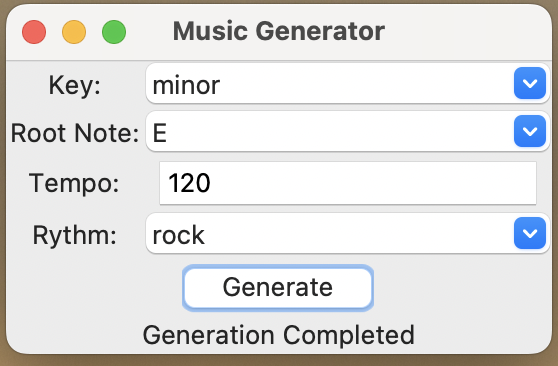
\includegraphics[width=1\textwidth]{/Users/leonardoangellotti/Desktop/università/terzo anno/tesi/MusicGeneticAlgorithm-main/genetic_music/final results rock/results/setting} 
    \caption{Descrizione dell'immagine}
    \label{fig:immagine}
\end{figure}

al termine dell'esecuzione vengono stampati i risultati dei punteggi ottenuti dalla fitness function, per i genomi di ogni popolazione.

% Inserimento di un'immagine
\begin{figure}[h!]
    \centering
    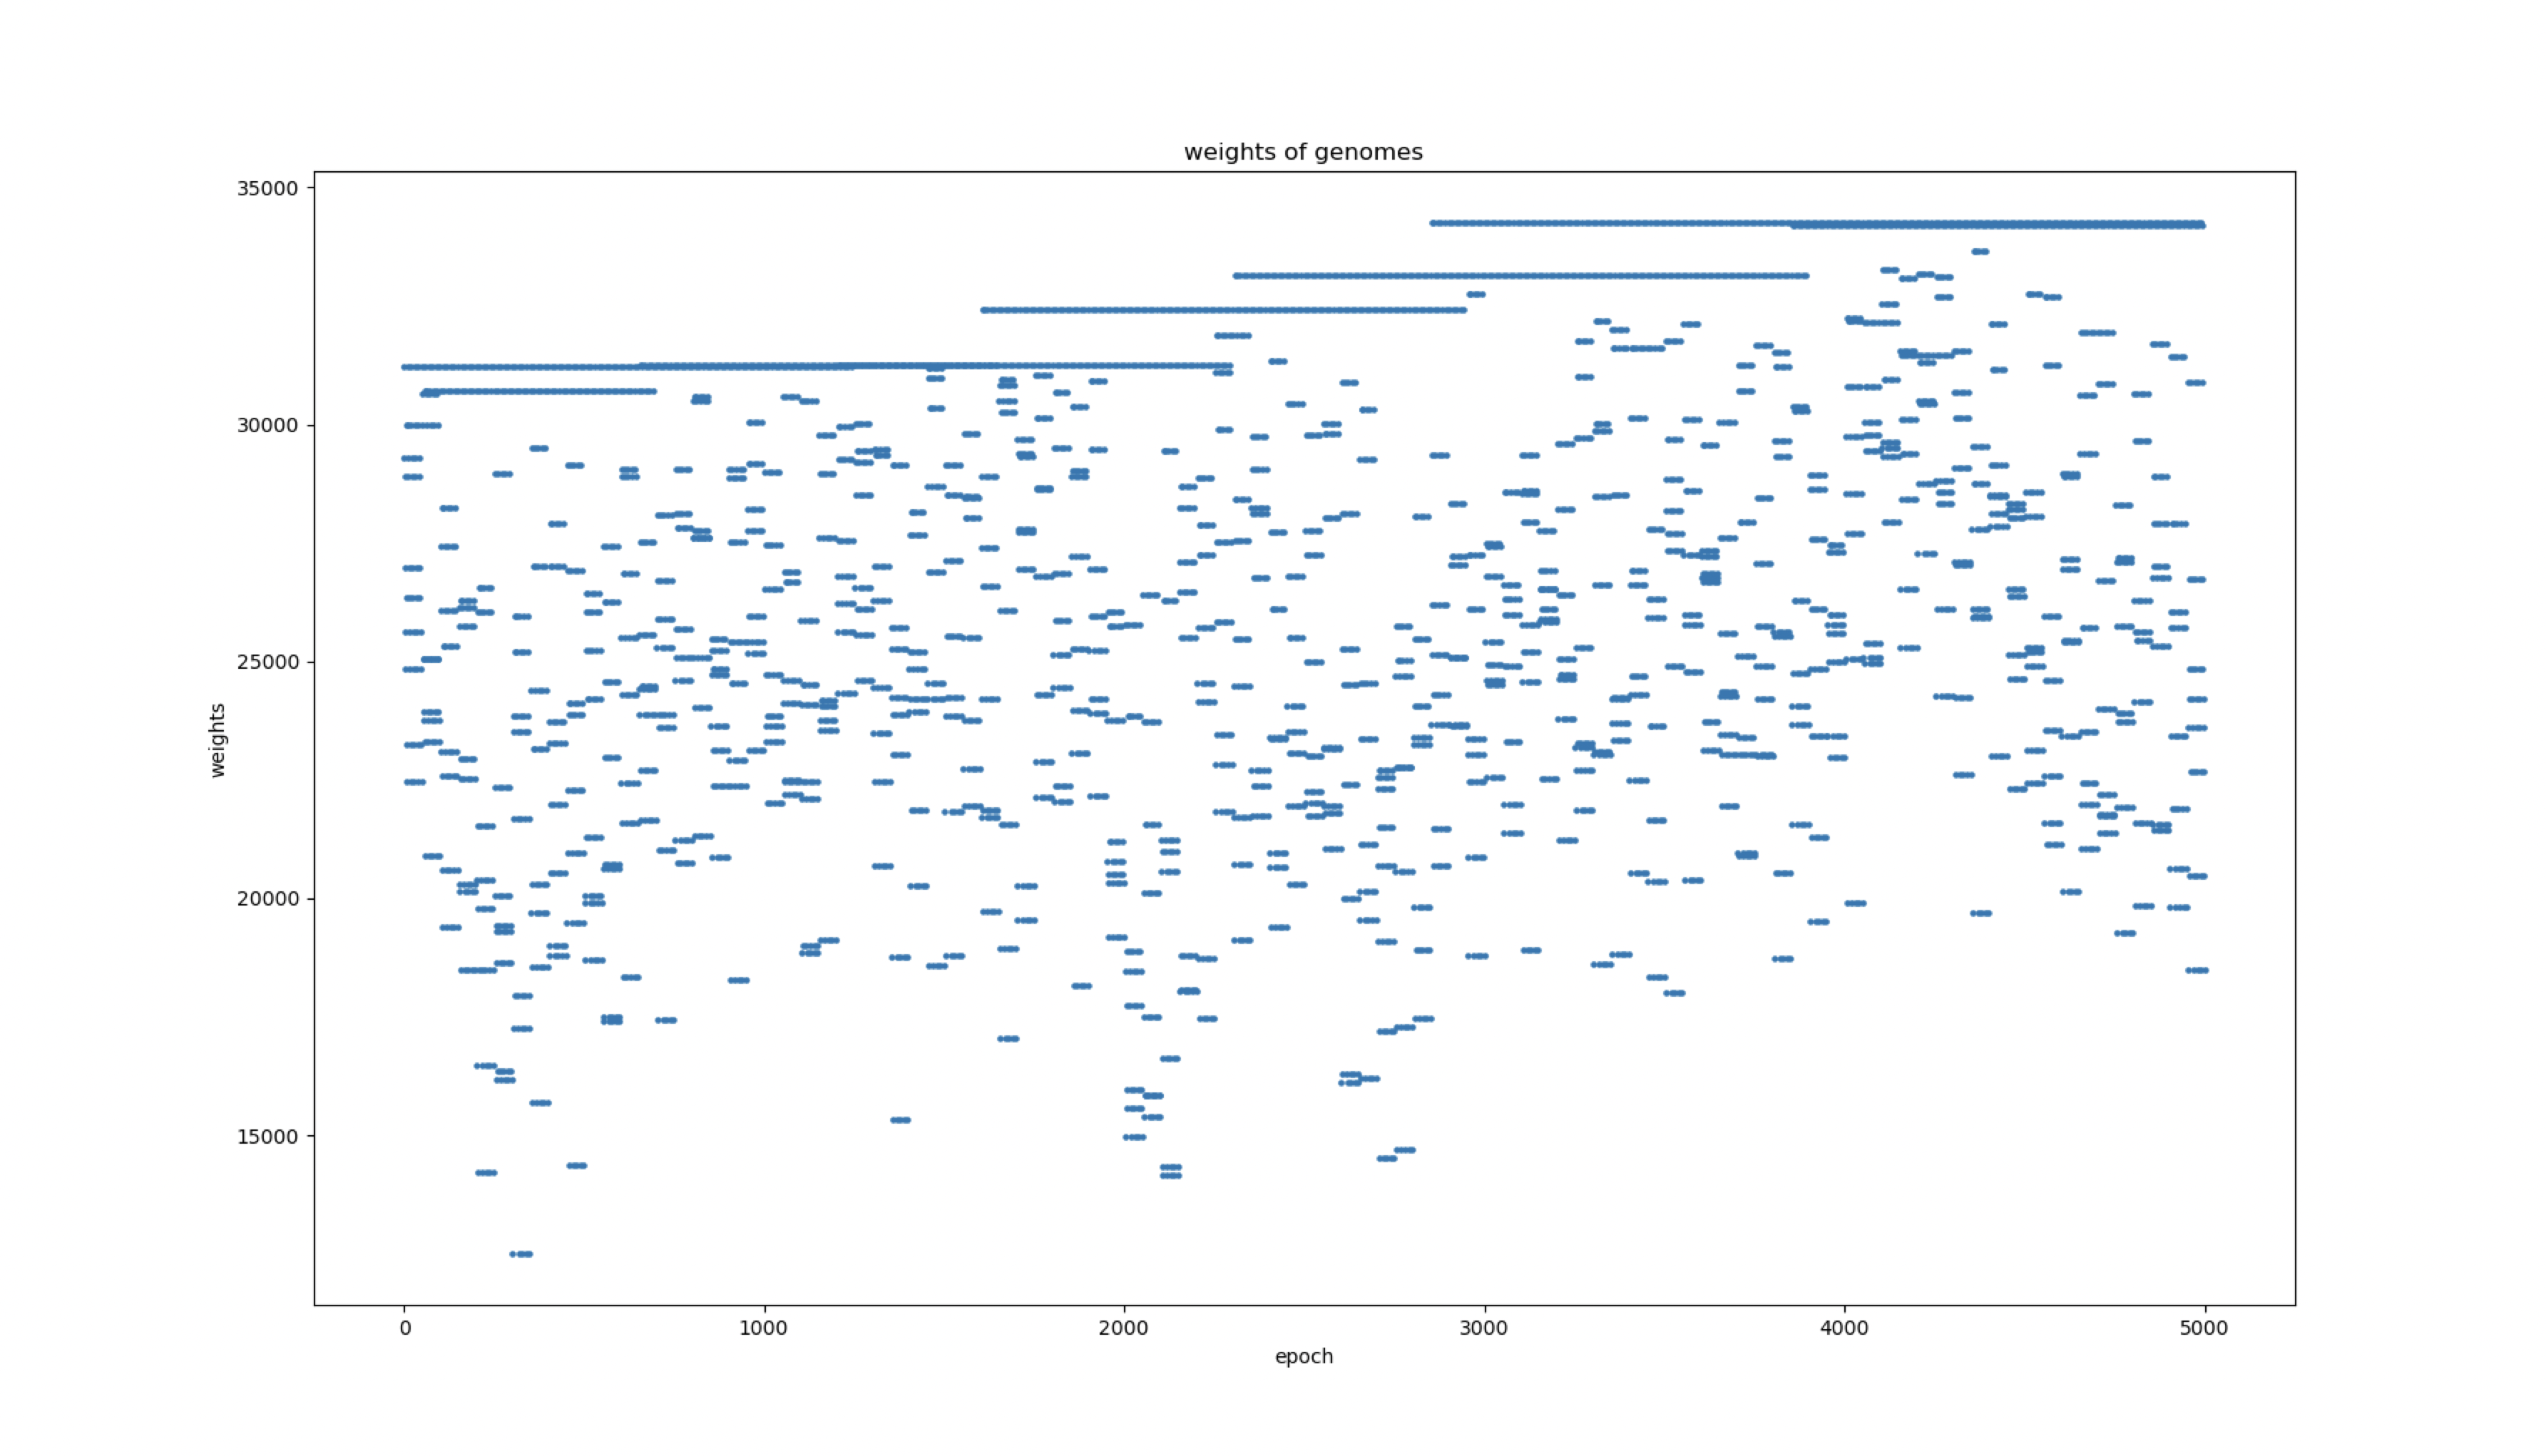
\includegraphics[width=1\textwidth]{/Users/leonardoangellotti/Desktop/università/terzo anno/tesi/MusicGeneticAlgorithm-main/genetic_music/final results rock/results/scores} 
    \caption{Descrizione dell'immagine}
    \label{fig:immagine}
\end{figure}

Le linee che si mantengono costanti sono i punteggi dei primi due genomi (con punteggio più alto ad ogni generazione) che nell'algoritmo scelto vengono tramandati senza alcuna alterazione (crossover, mutation).
Quando "nasce" un nuovo genoma che si verifica avere un punteggio più altro dei primi due, questo fissa un nuovo livello di punteggio superiore ai precedenti, che viene mantenuto finché ciò non accade nuovamente.
Questa procedura garantisce un costante aumento del punteggio e un conseguente miglioramento tra le popolazioni.
La nuvola di punti che appaiono al di sotto, con punteggio inferiore, appartengono al set di genomi soggetti a crossover e mutazioni.

Al termine della procedura evolutiva, vengono stampati i 10 genomi appartenenti all'ultima popolazione.

% Inserimento di un'immagine
\begin{figure}[h!]
    \centering
    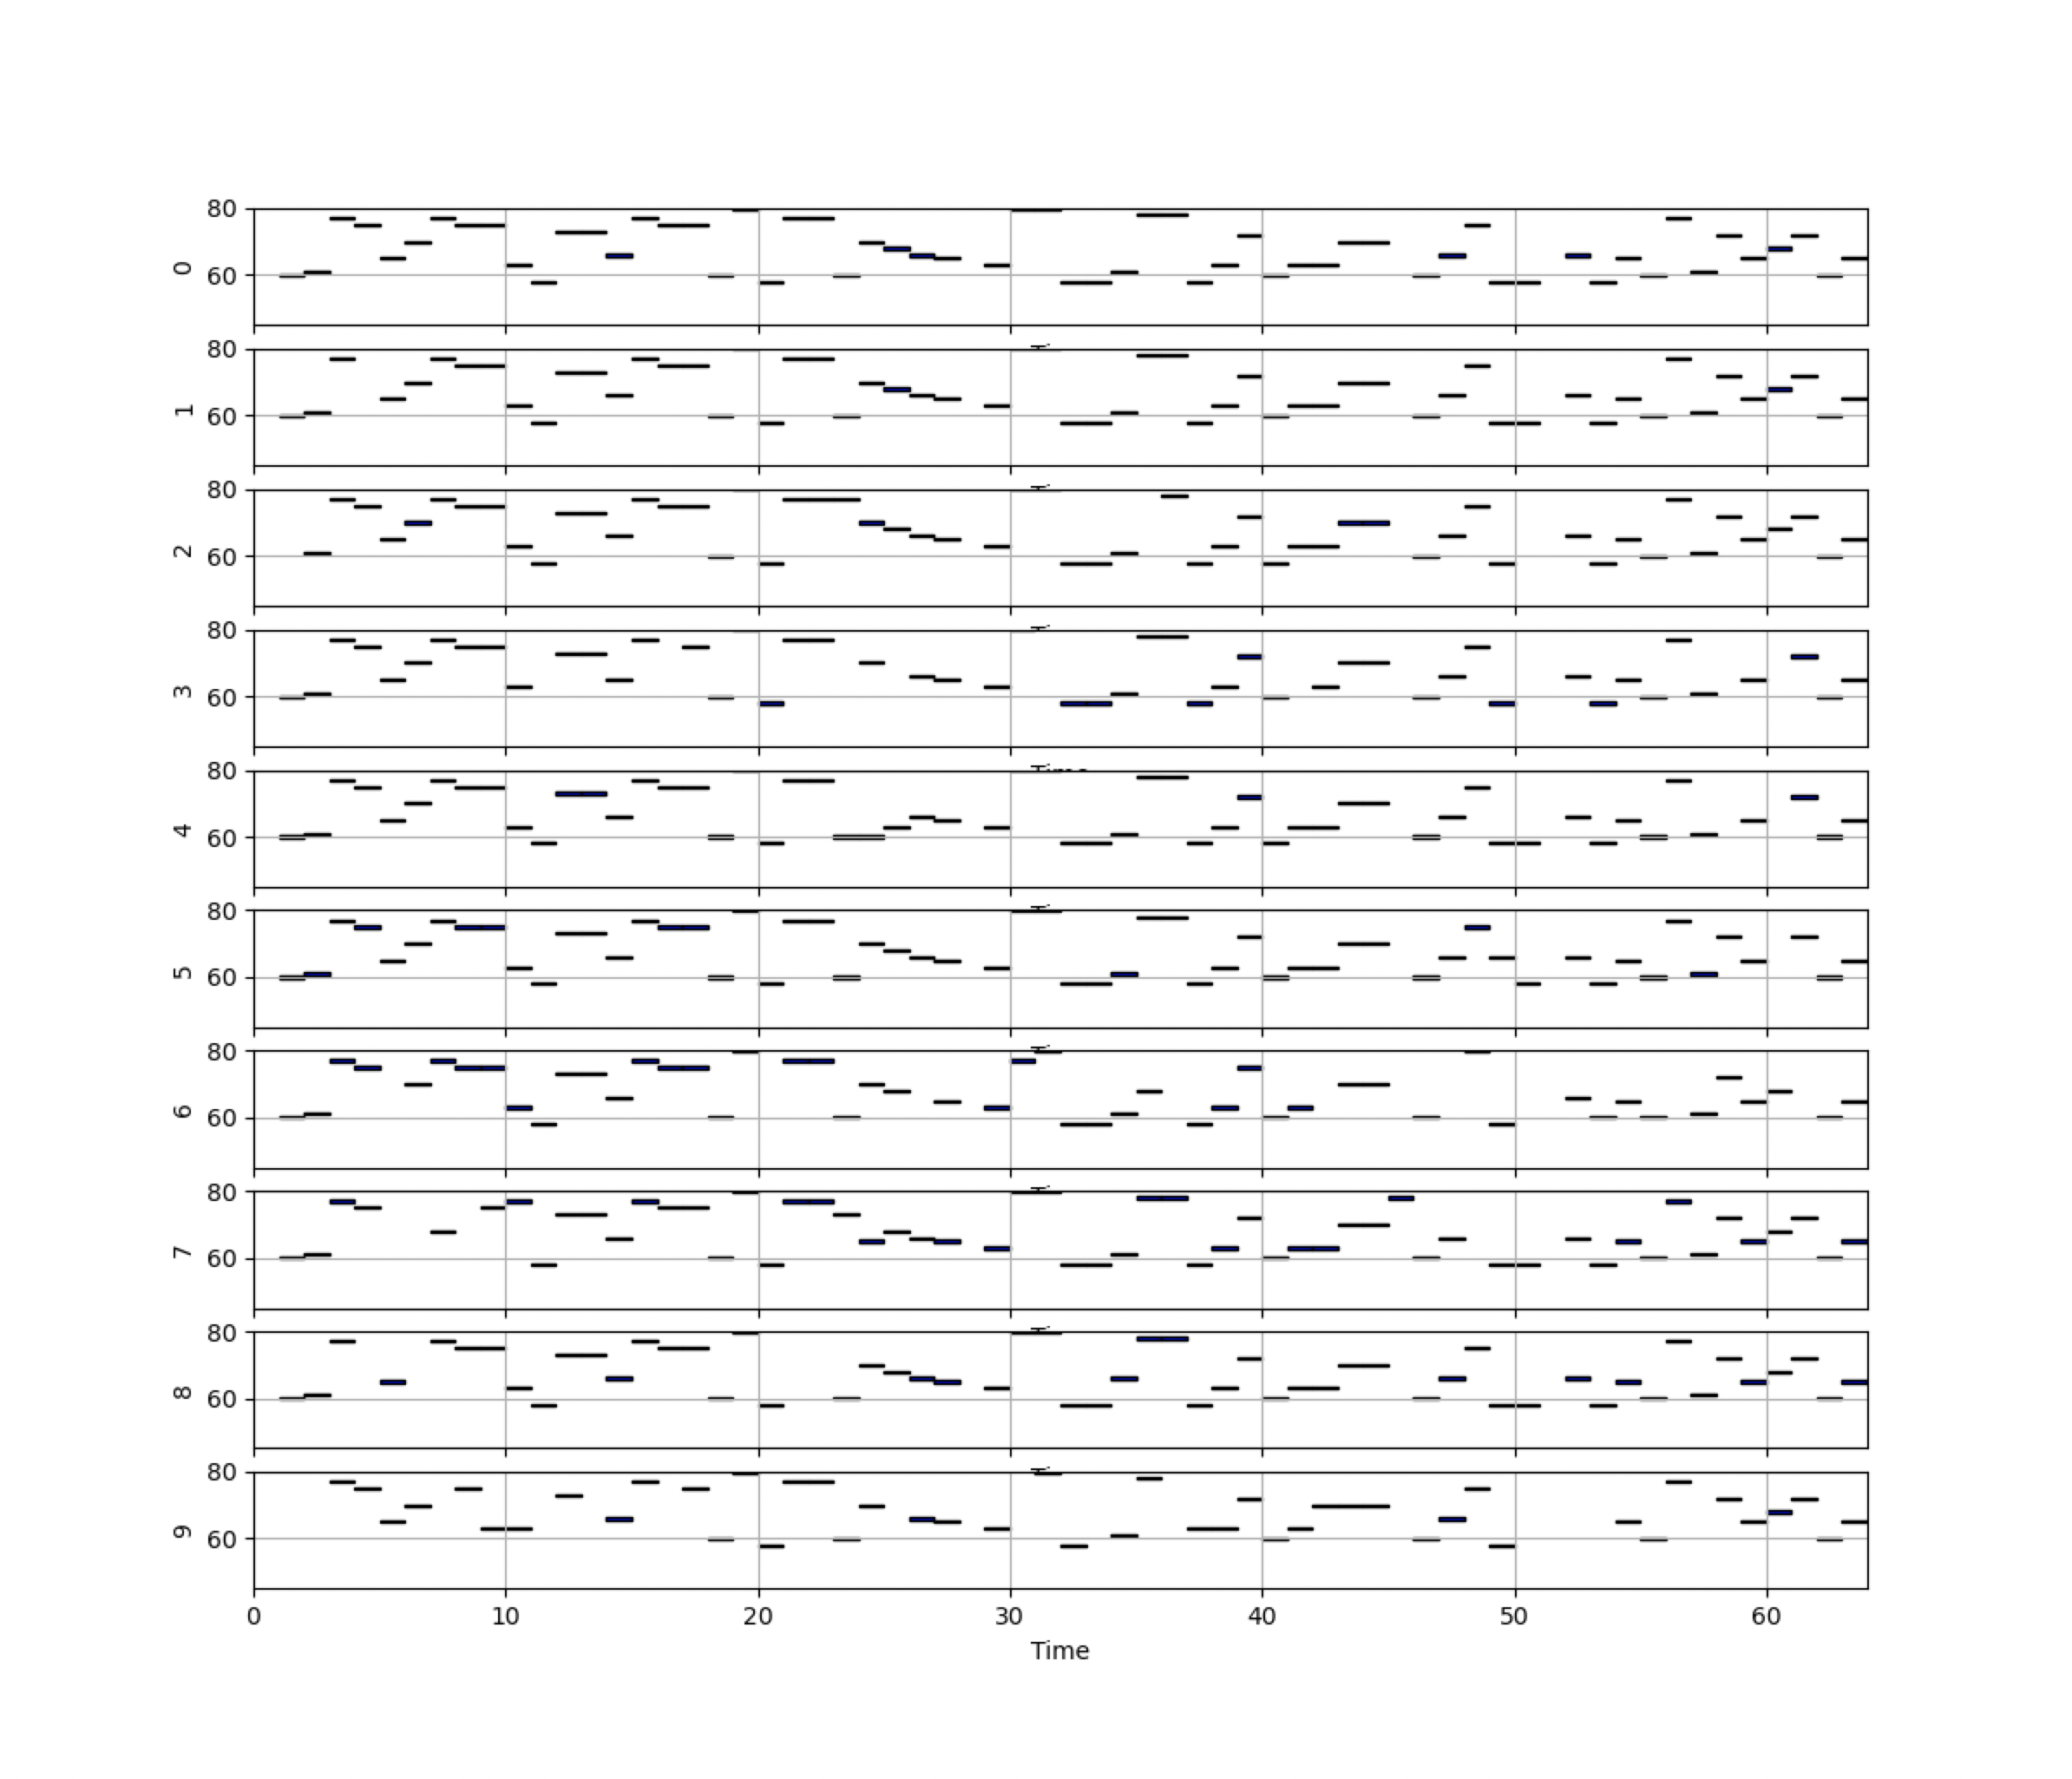
\includegraphics[width=1\textwidth]{/Users/leonardoangellotti/Desktop/università/terzo anno/tesi/MusicGeneticAlgorithm-main/genetic_music/final results rock/results/MIDI} 
    \caption{Descrizione dell'immagine}
    \label{fig:immagine}
\end{figure}

La stampa rappresenta 10 file midi, dal migliore (numero 0) al "peggiore" (numero 9) secondo la nostra fitness-function.
Le note sono rappresentate dalle linee orizzontali che appaiono a diverse altezze di pitch, indicati nell'asse delle ordinate.
Le note sono sequenziali, appaiono dunque in momenti consecutivi, con diversa durata (dettata dal ritmo scelto dall'utente)
Si ricorda che l'algoritmo genera una sequenza monofonica, infatti non appare più di una nota contemporaneamente.

Le sequenze vengono salvate su disco. 
Il genoma migliore prende il nome di best_genome.mid, mentre ai restanti viene assegnato un numero in ordine decrescente in punteggio (genome_0.mid, ..., genome_8.mid).

Ad un primo ascolto di best_genome.mid, percepiamo un movimento coerente nella teoria, ordinato nel ritmo, ma non regolare nel tempo. 
Non viene percepita infatti alcuna vera struttura compositiva, questo perché la fitness function si è preoccupata di fare confronti solo tra una nota e la precedente, e non tra tutte le note della sequenza.
Non esiste dunque una vera struttura a lungo termine, una struttura narrativa, avente inizio svolgimento e fine, propria invece di qualsiasi genere musicale.
Non è presente nemmeno il classico schema delle canzoni pop: verso-ritornello-verso-ritornello-bridge-ritornello.

Per ovviare a questo difetto si procedere con un'operazione naive ma efficace:
Si decide di generare una nuova sequenza, chiamata repeated_melody.mid, la quale ripete per 4 volte le prime 3 bar prese dal best_genome.mid.
Il risultato risulta essere "ripetitivo" e dunque intrinsecamente più regolare, oltre a essere per il nostro orecchio più confortevole.

Abbiamo dunque ottenuto un risultato teorico "accettabile" e coerente. 
Possiamo ottenere di più nella pratica?
Si.
Importando il file midi (repeated_melody.mid) in una DAW (Digital Audio Workstation, in questo caso è stato utilizzato Ableton) possiamo apportare ulteriori modifiche.
Viene assegnata alla traccia lo strumento Grand Piano. 
Sue questa vengono applicate le seguenti opzioni

% Inserimento di un'immagine
\begin{figure}[h!]
    \centering
    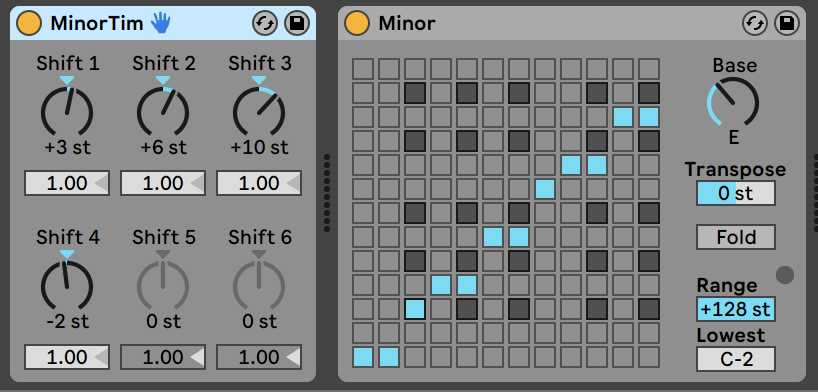
\includegraphics[width=1\textwidth]{/Users/leonardoangellotti/Desktop/università/terzo anno/tesi/MusicGeneticAlgorithm-main/genetic_music/final results rock/results/ableton_settings} 
    \caption{Descrizione dell'immagine}
    \label{fig:immagine}
\end{figure}

"MinorTim" permette di generare più note, ad una certa distanza in semitoni, partendo dalla nota corrente. 
Nel caso specifico un accordo minore.
Tuttavia un primo ascolto risulta essere poco piacevole, perché le note generate non considerano la scala di riferimento.
È necessario dunque usare lo strumento "Minor" per ancorare ogni nota in una posizione coerente.
Il risultato è decisamente più armonico, seppur tuttavia ancor troppo "piatto" con nessuna variazione nell'esecuzione.
Per far fronte a questa "freddezza" ed aumentare la dinamicità è possibile randomizzare, in modo automatico, i valori di Velocity nella sequenza per ciascuna nota.
Un nuovo ascolto ci ricorda un qualche compositore jazz, immerso nel suo fiume di sentimenti, vissuti istante per istante, 
ma che vuole comunque mantenere, per piacere della clientela, un ritmo e melodia regolari.

Per rendere il risultato ancor più gradevole, e musicalmente completo, possiamo aggiungere un elemento di percussioni, come una batteria.
Per il risultato ottenuto è stato utilizzato il plug-in Magenta (https://magenta.tensorflow.org/studio) sviluppato da Google e attualmente disponibile gratuitamente.
In particolare è stato utilizzata la funzione "Drumify", che data una sequenza di note, genera un secondo file MIDI in cui, similmente per il piano, vengono indicate le parti della batteria da percuotere (piatto, charleston, gran cassa, rullante).
In particolare, nel risultato finale, quest'ultima sequenza MIDI è stata processata dal Plugin SuperiorDrummer3 (https://www.toontrack.com/product/superior-drummer-3/?gad_source=1&gclid=Cj0KCQjws560BhCuARIsAHMqE0H2FsGI5sBj5JLtPNhhiKiLf9qMEccOntk8F9uc4_ZvSDPK5TCZZKUaAg1LEALw_wcB),
una libreria sofisticata che raccoglie suoni di batteria accurati.
Si vuole far notare, che l'algoritmo implementato in Drumify, si basa su una neural network, non è di tipo genetico come nel caso del nostro esempio, in grado dunque di cogliere e sviluppare una certa consequenzialità tra parti.

Infine, per le basse frequenze è stata aggiunta una semplice linea di basso, trasponendo la melodia due ottave inferiori, eliminando a mano, secondo il propio gusto, le note ridondanti, lasciando invece quelle fondamentali e di maggiore durata.

Il risultato finale, nello specifico, è "quasi" accettabile, considerando che per generarlo sono state necessarie poco più di 500 linee di codice (commenti inclusi) e qualche plugin dal mondo di internet.
Il tratto fondamentale risiede nel fatto che per ottenere questo file mp3, non abbiamo mai: né dovuto suonare un pianoforte, slappare un basso o ritmare una batteria a tempo.

Si possono sperimentare ulteriori modifiche, cambiando i pesi (smoothnessWeight, restWeight, harmonyWeight) o implementando un sistema nell'assegnazione della durata e velocity nelle note, ora affidate ad array con valori prefissati (rock, jazz, dance, bossa nova) e ad una scelta random rispettivamente.

\chapter{Conclusioni}

Negli ultimi decenni, la ricerca sulla generazione musicale ha compiuto enormi progressi nella generazione di aspetti ben definiti della musica come la melodia, l’armonia, il ritmo e il timbro. 
Modelli statistici all’avanguardia, tecniche di ottimizzazione avanzate, database digitali più grandi su cui addestrare i modelli e l’aumento della potenza di calcolo hanno portato alla produzione di sistemi migliori. 

Perché allora non utilizziamo sistemi di generazione musicale nella nostra vita quotidiana? 

L’indagine di cui sopra mostra che rimane un’importante sfida generale: quella di creare musica con una struttura a lungo termine.

La struttura a lungo termine, che spesso assume la forma di temi, motivi e schemi ricorrenti, è una parte essenziale di qualsiasi esperienza di ascolto musicale. In secondo luogo, gli sviluppi nel campo del deep learning mostrano che le reti neurali possono incorporare strutture di memoria durante l'apprendimento di dati sequenziali. 

Per rendere i sistemi musicali generati dal computer parte della nostra vita quotidiana, c’è bisogno di sistemi più “narrativi", in grado cioè di creare un inizio, sviluppo e conclusione nella musica. 

Sebbene ci siano recenti tentativi di generare musica con tensione [Farbood et al. 2007; Herremans e Chew 2016a], che sia applicata a colonne per videogiochi o che accompagnano film, c’è ancora margine di miglioramento per comprendere meglio la connessione tra musica ed emozione, 
in modo da integrare questa relazione cruciale nei sistemi di generazione musicale. 

Ciò potrebbe portare ad applicazioni pratiche nella vita reale, come la generazione di musica in tempo reale.

Sebbene le tecniche di apprendimento automatico possano essere estremamente utili in compiti come la già citata modellazione delle emozioni nella musica, di solito richiedono grandi quantità di dati. 

Pertanto, il settore ha riscontrato una continua necessità di ulteriori dati. 
Esiste un potenziale reale affinché il lavoro futuro si sposti verso sistemi intelligenti che non richiedano abbondanti quantità di dati, capaci di un ragionamento innato rispecchiando meglio il funzionamento della mente umana. 
Ciò risolverebbe anche la continua sfida di trovare un equilibrio tra la rigenerazione della musica esistente e i frammenti di questa senza ricadere nel plagio.

Una delle caratteristiche della musica generata dal computer che viene spesso trascurata è la difficoltà di esecuzione. 
Mentre un'applicazione potrebbe essere quella di adattare la nuova musica a un certo livello di abilità del musicista, esiste anche la possibilità di utilizzare la difficoltà di esecuzione rilevata/calcolata come misura di valutazione per la musica generata.

Rimane difficile, tuttavia, confrontare oggettivamente sistemi diversi poiché di solito accettano parametri di input diversi, generano aspetti musicali diversi, sono addestrati su stili diversi o non hanno esempi audio disponibili per il lettore. Inoltre, negli esperimenti di ascolto, l’effetto di mera esposizione [Zajonc 1968] farà sì che gli ascoltatori preferiscano i brani esistenti rispetto a quelli nuovi, poiché la familiarità provoca un maggiore godimento.

\appendix
\chapter{Appendice A}
\section{Dettagli aggiuntivi}

\chapter{Appendice B}
\section{Altro materiale supplementare}

% Esempio di citazione
Come descritto da Lamport \cite{latex}, e come discusso da Doe e Smith \cite{example_article}, i metodi utilizzati sono basati su...

% Bibliografia
\bibliographystyle{plain}
\bibliography{bibliografia}

\end{document}
